\chapter{Materiais e M�todos}
\label{Materiais}

\textcolor{red}{\textbf{Dica:} Materiais e M�todos: descri��o clara dos procedimentos e dos materiais
adotados para o desenvolvimento do trabalho (sem resultados) ? incluindo sua
adequa��o ao trabalho.
Tem que responder �s perguntas:
-est� com um tamanho adequado (proporcional) � monografia?
-h� informa��o suficiente e clara sobre os materiais e sobre os m�todos
adotados?
N�o h� necessidade de reproduzir (copiar) as obras que embasam o trabalho e
sim colocar o suficiente para o entendimento do trabalho e citar as refer�ncias.}


%------------------------------------ Materiais -----------------------------------------------------
\section{Materiais}

\begin{figure}[H]
 	\centering
 	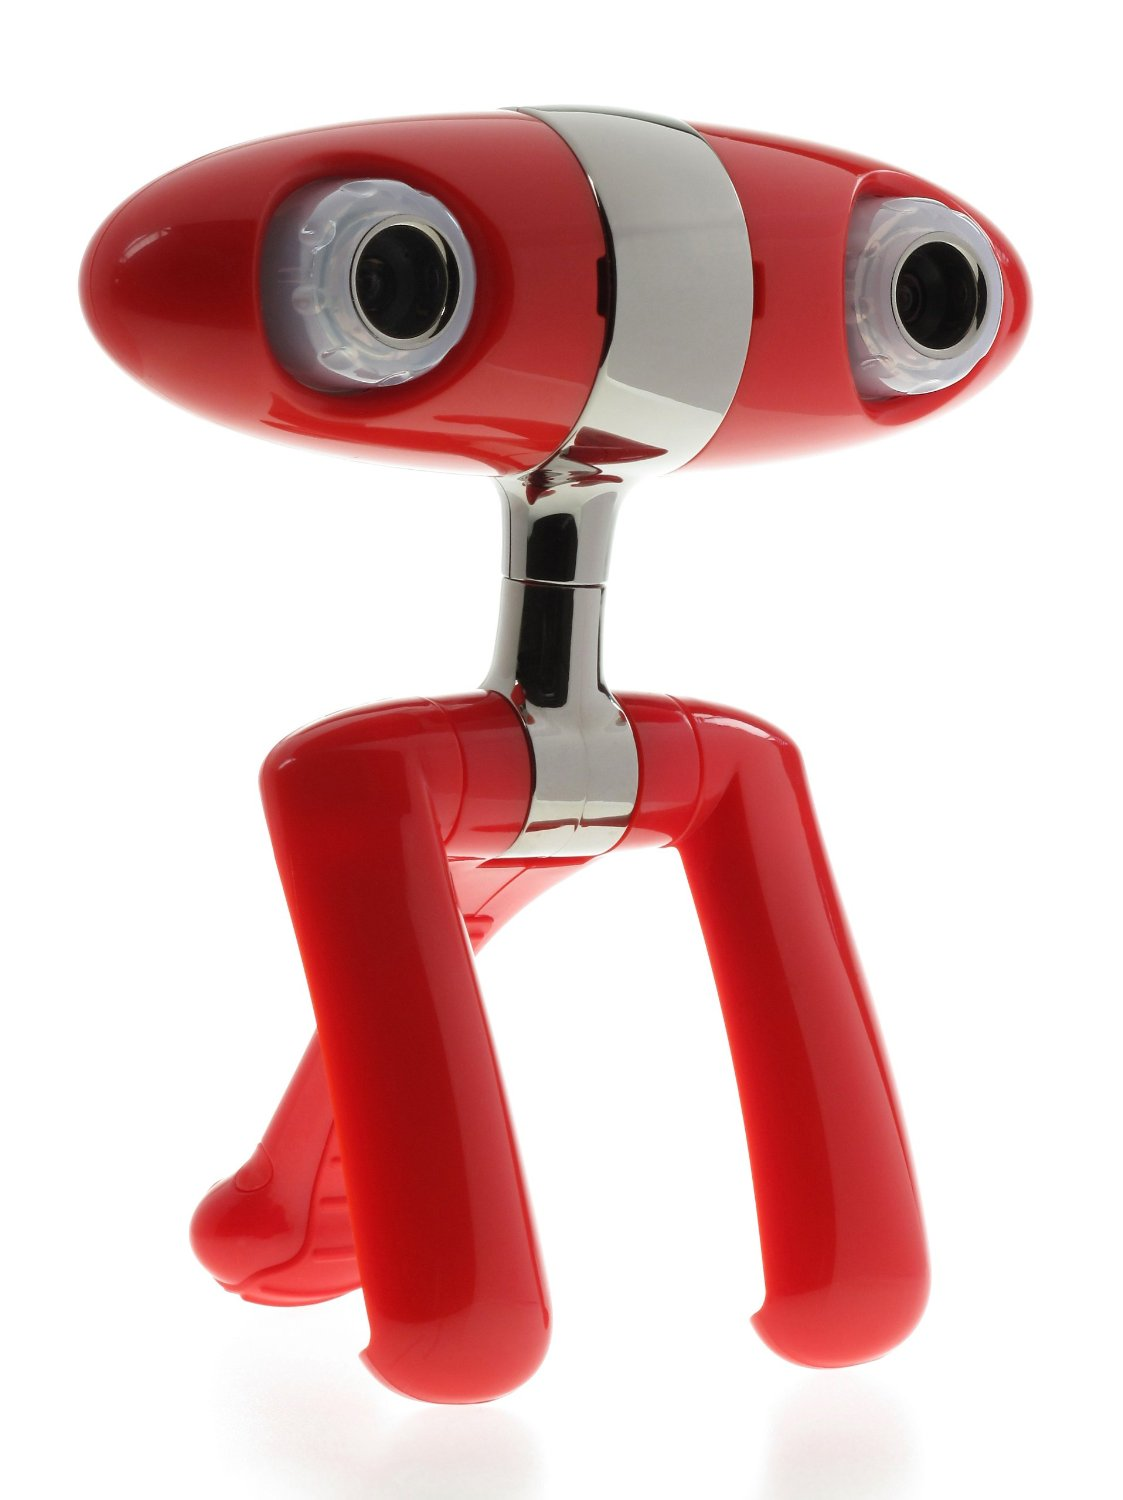
\includegraphics[scale=0.10]{./Resources/minoru.jpg}
 	\caption{3D Webcam Minoru}
 	\label{minoru}
\end{figure}

\begin{figure}[H]
 	\centering
 	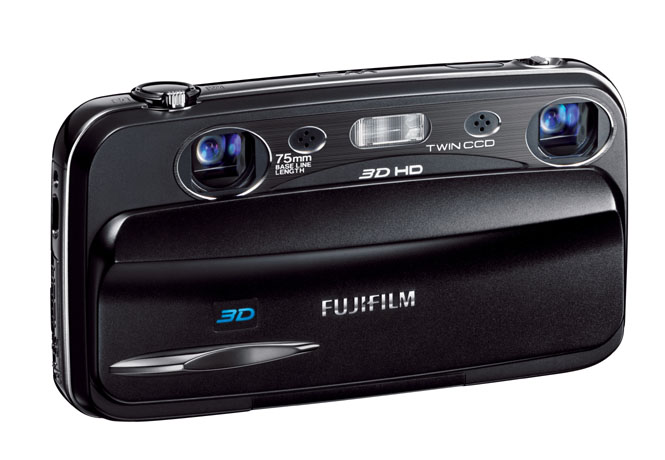
\includegraphics[scale=0.35]{./Resources/fujiW3.jpg}
 	\caption{C�mera Digital Fujifilm FinePix Real 3D W3}
 	\label{fujiW3}
\end{figure}

\begin{figure}[H]
 	\centering
 	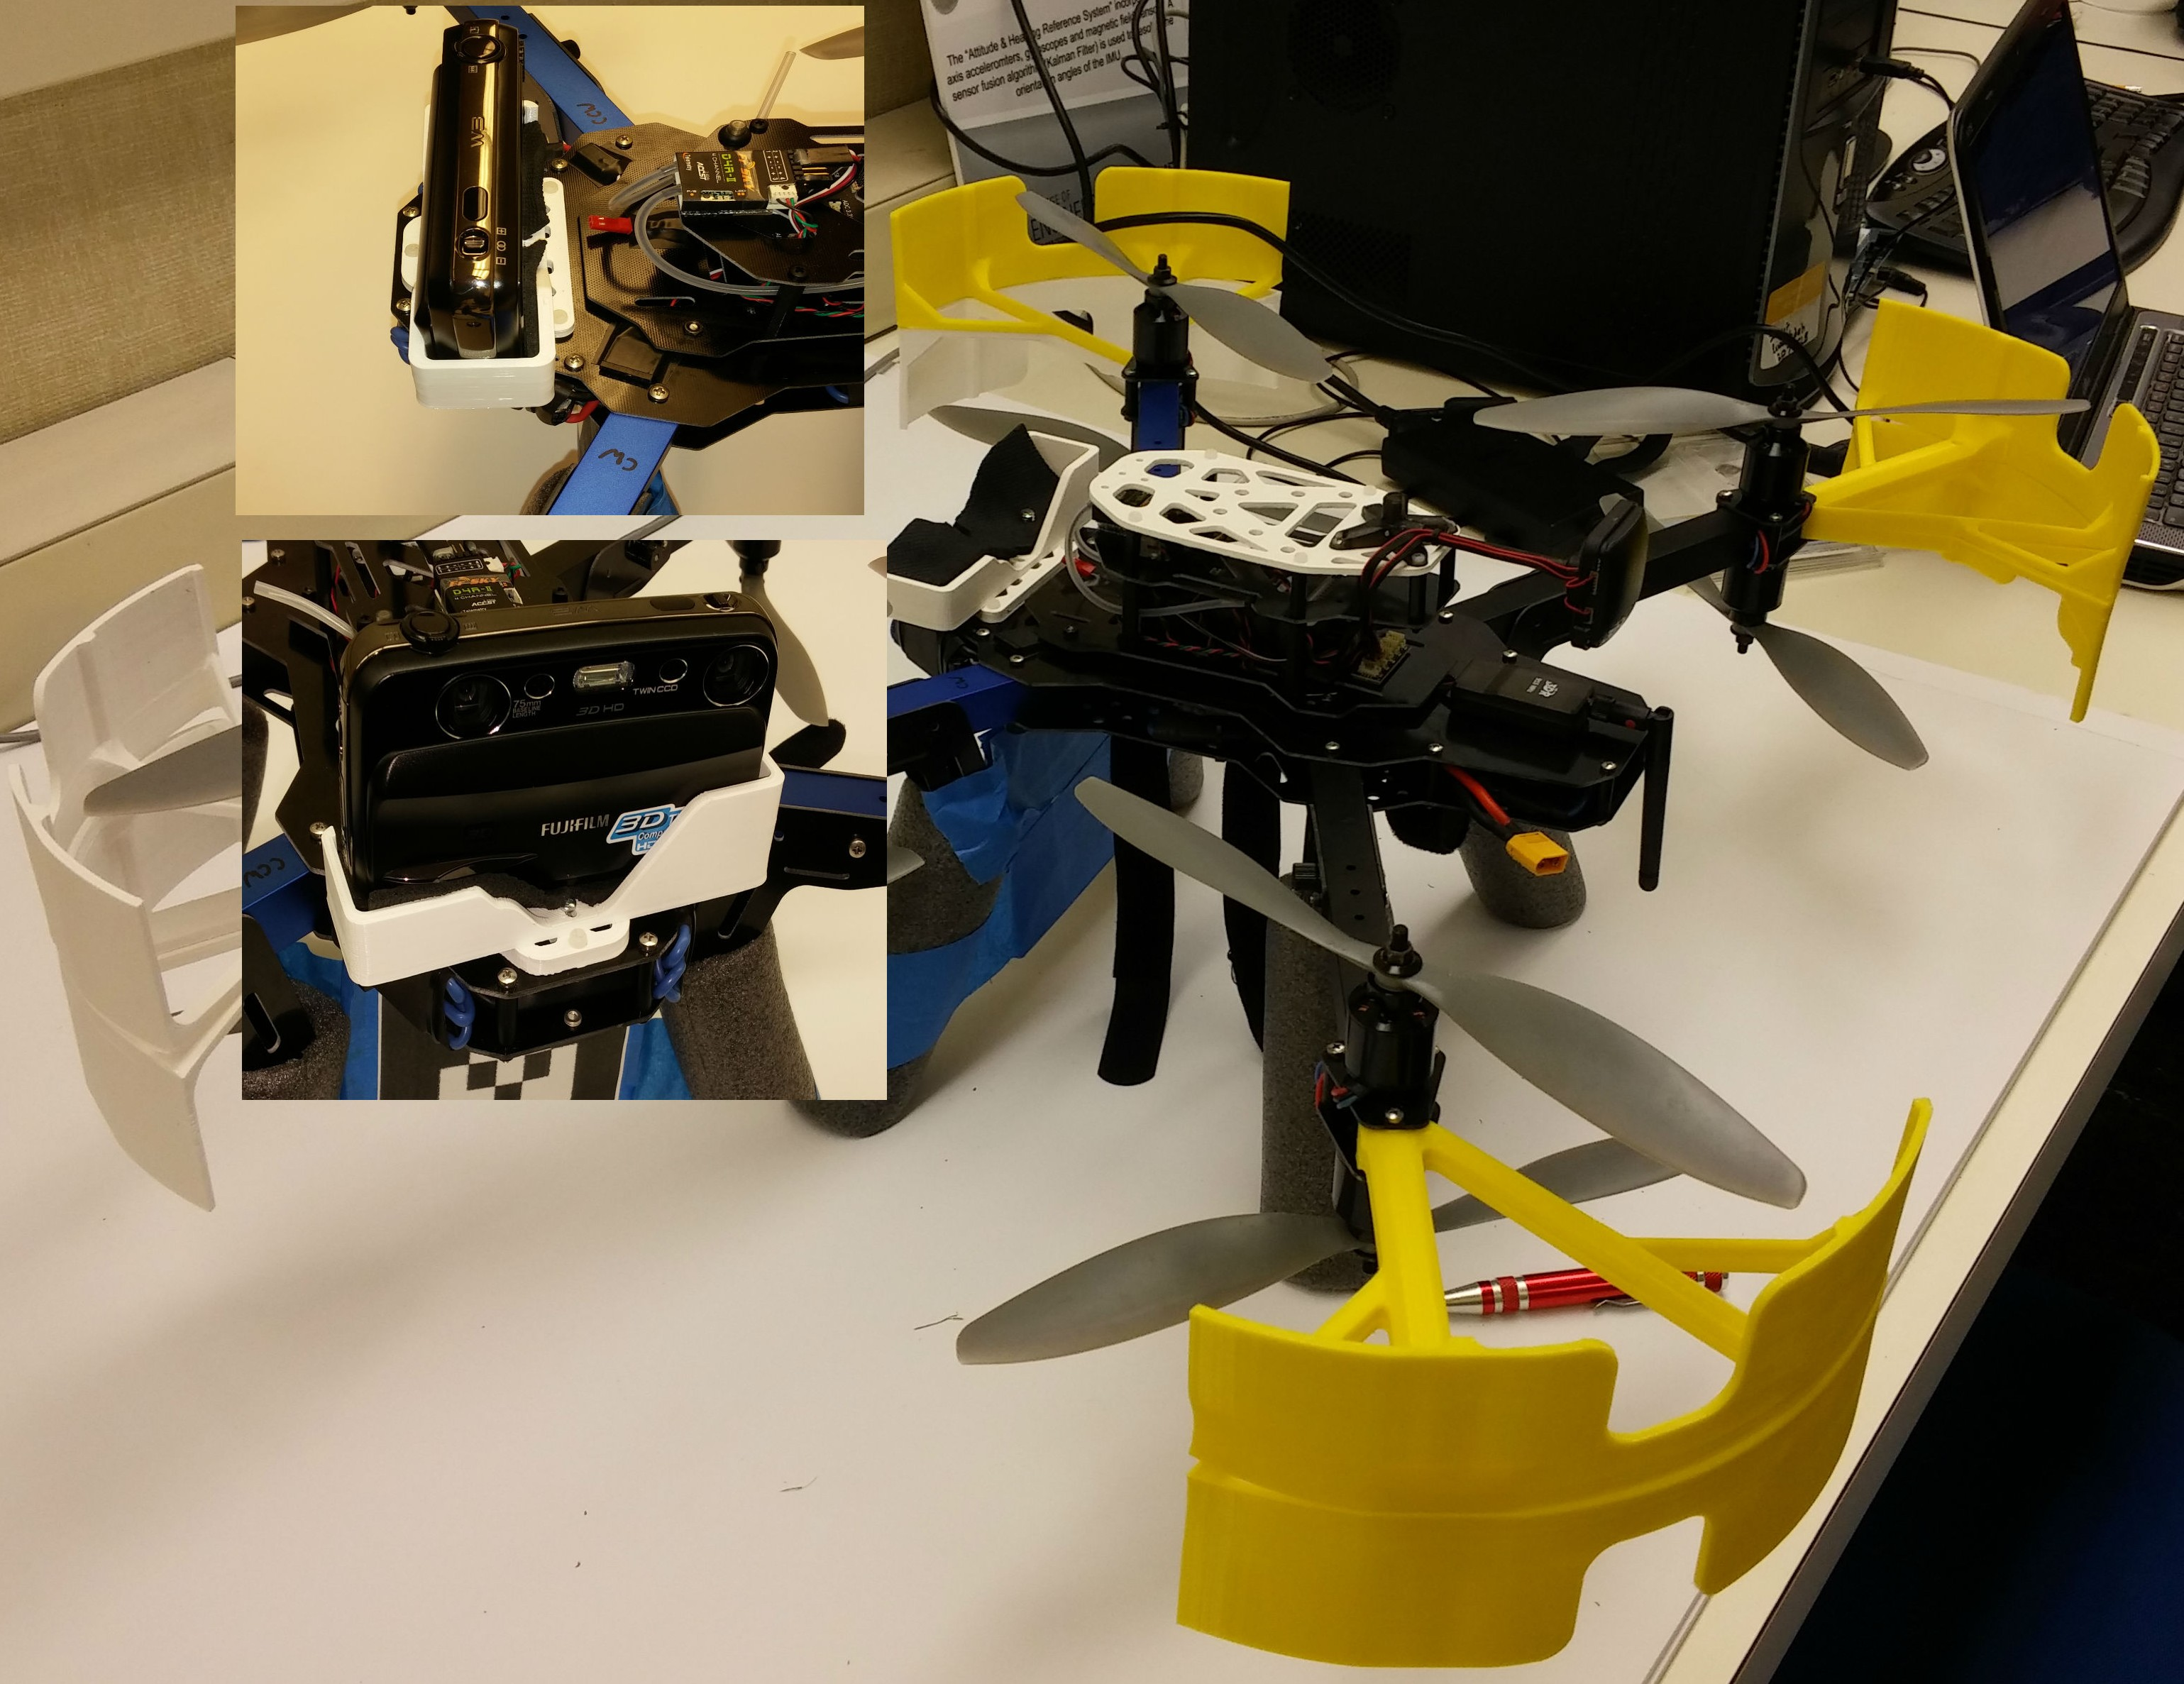
\includegraphics[scale=0.10]{./Resources/quad_camera_support.jpg}
 	\caption{Quadric�ptero 3DR X8 com suporte para a C�mera 3D}
 	\label{quad_camera_support}
\end{figure}

Capture high-resolution images in 2D and 3D
Record HD 3D movies (720p resolution); dual 10-megapixel CCD and lens system
3.5-inch widescreen autostereoscopic LCD displays images and movies in 3D instantly, with no glasses required
mini-HDMI output jack offers easy connection to a compatible 3D HDTV; view images and movies instantly in 3D
Capture images and movies to SD/SDHC memory cards (not included)


%------------------------------------ M�todos -------------------------------------------------------
\section{M�todos}

M�todos utilizados no projeto.



